\chapter{Database}
The database model of resource management system consists of 10 entities, and 12 relations. 
\begin{figure}[H]
    \centering
    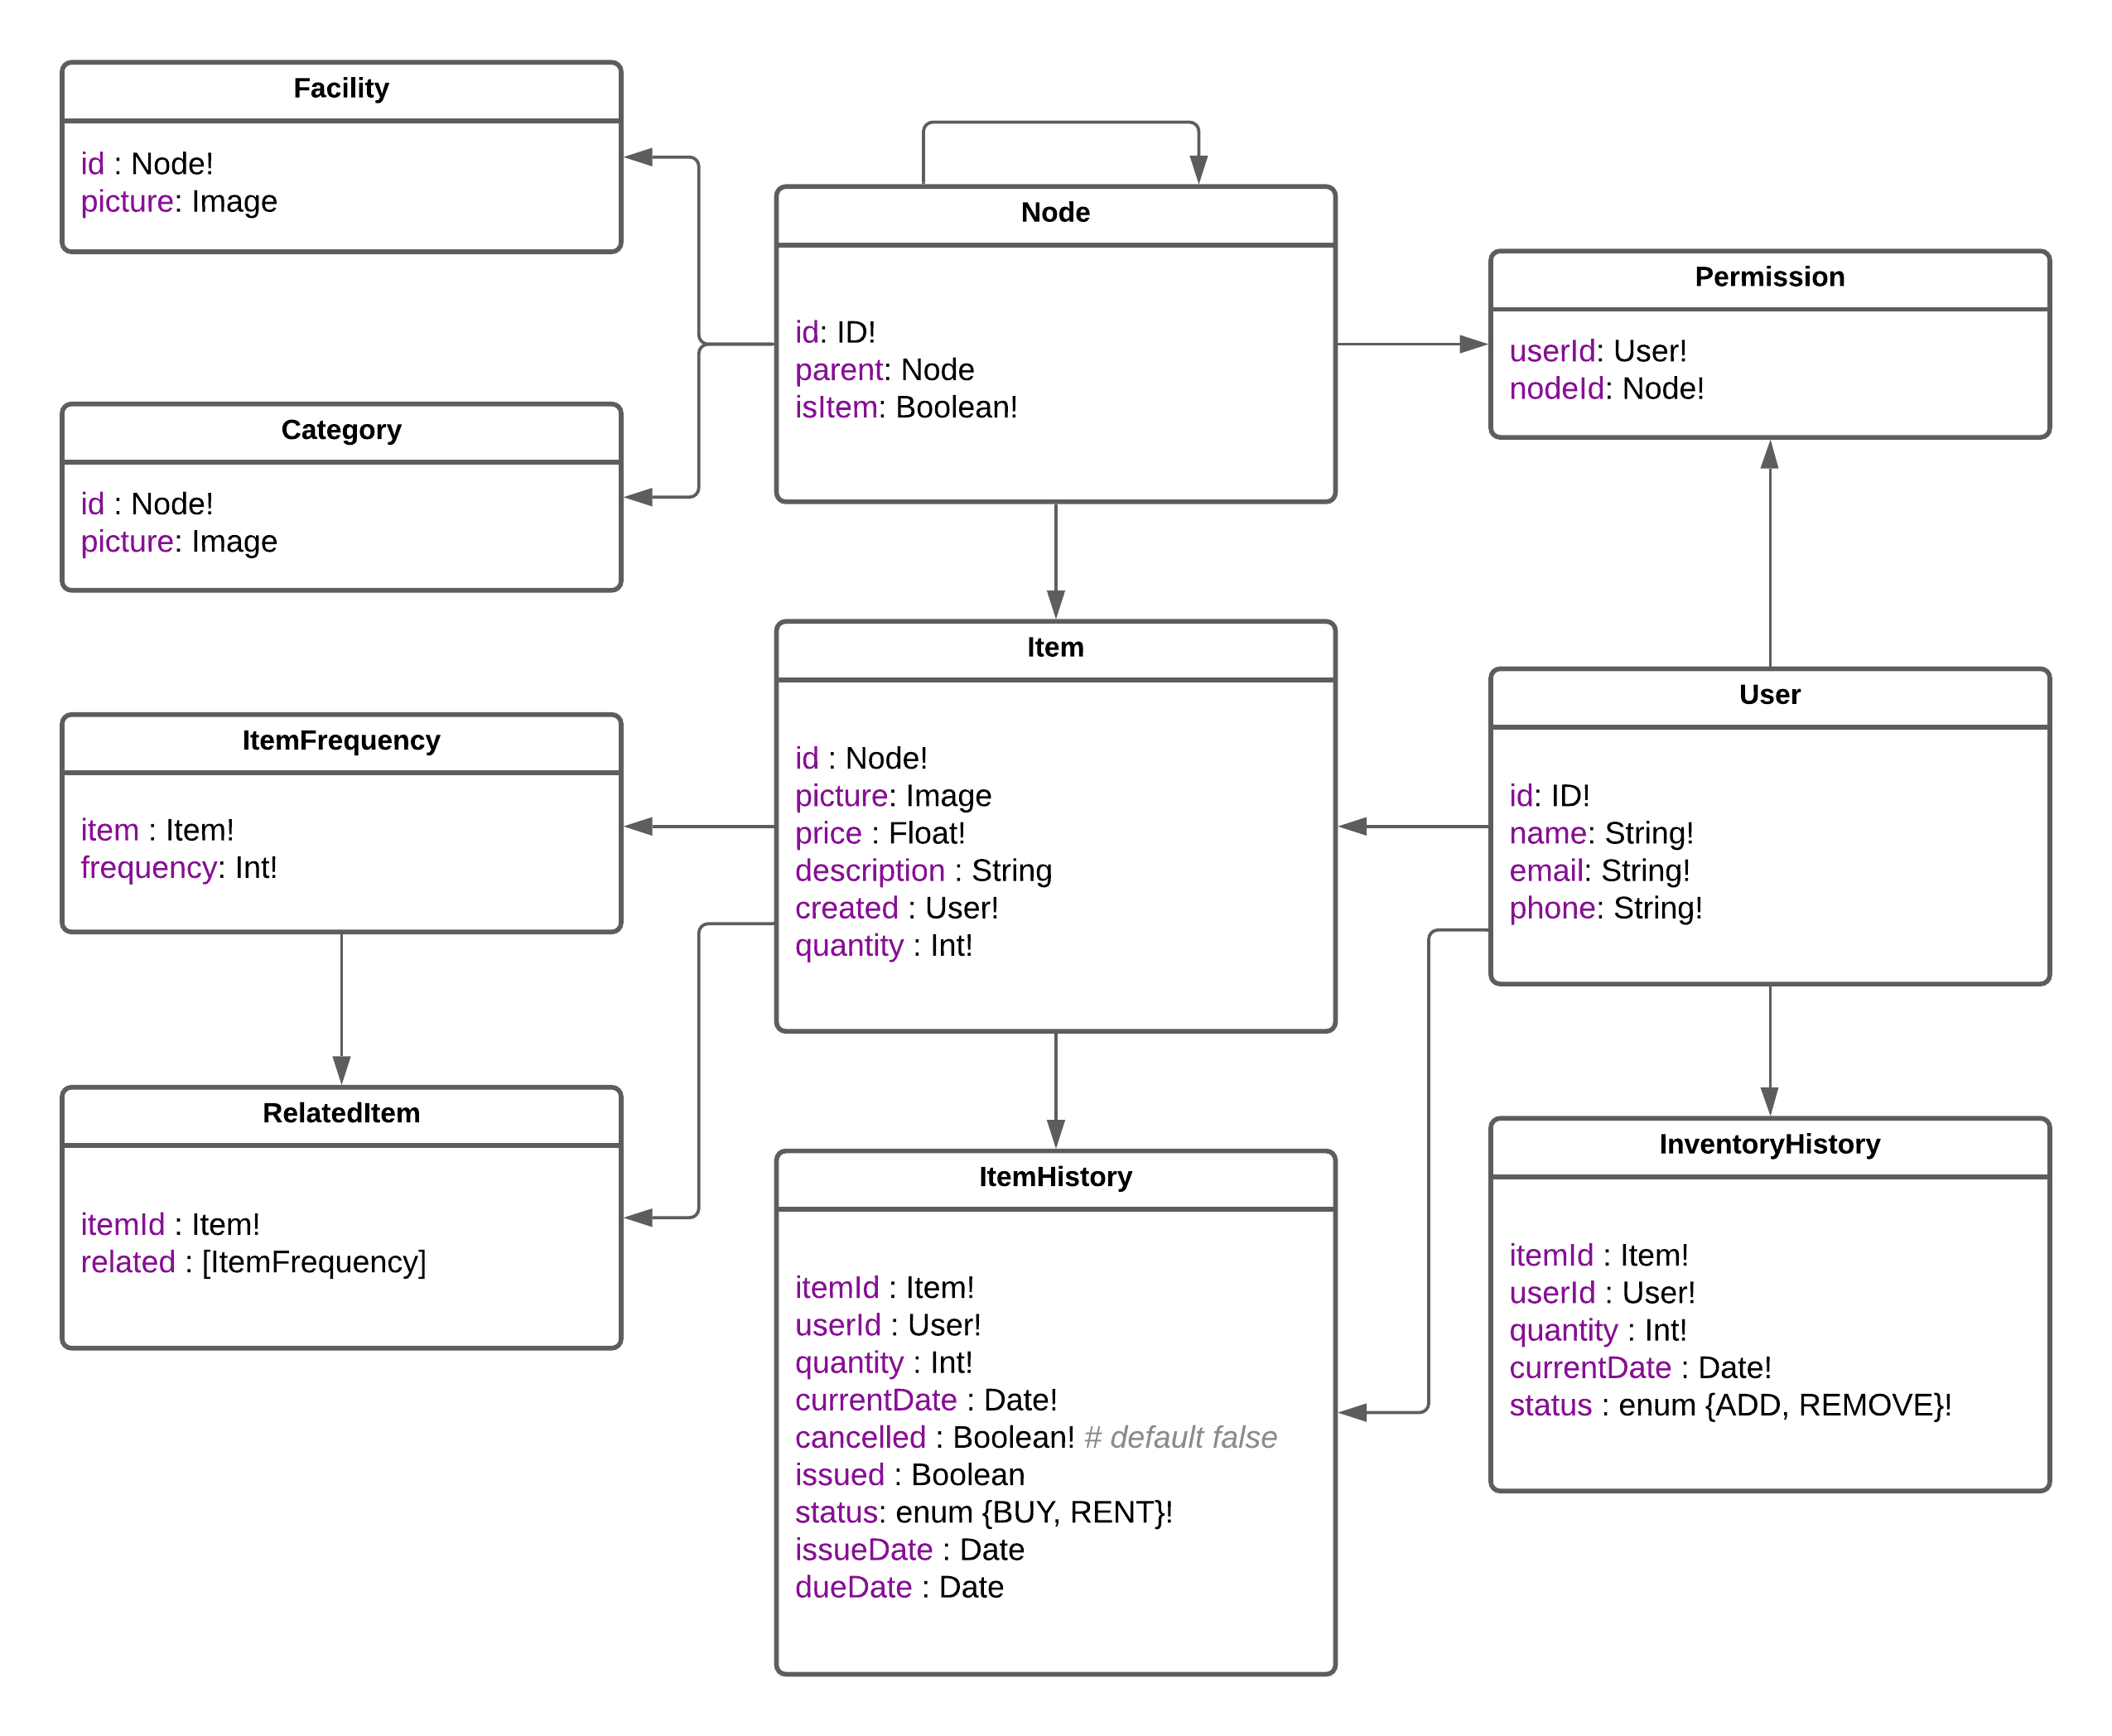
\includegraphics[scale=0.12]{images/schema.png}
    \caption{Database diagram}
    \label{fig:schema}
\end{figure}
\clearpage
Node is the central entity of the application. A nodes is either a facility, a category or an item. The application follows a forest data structure with each facility being a tree. The root of the tree is a facility with the leave nodes as the item and others category as shown in the figure below.
\begin{figure}[H]
    \centering
    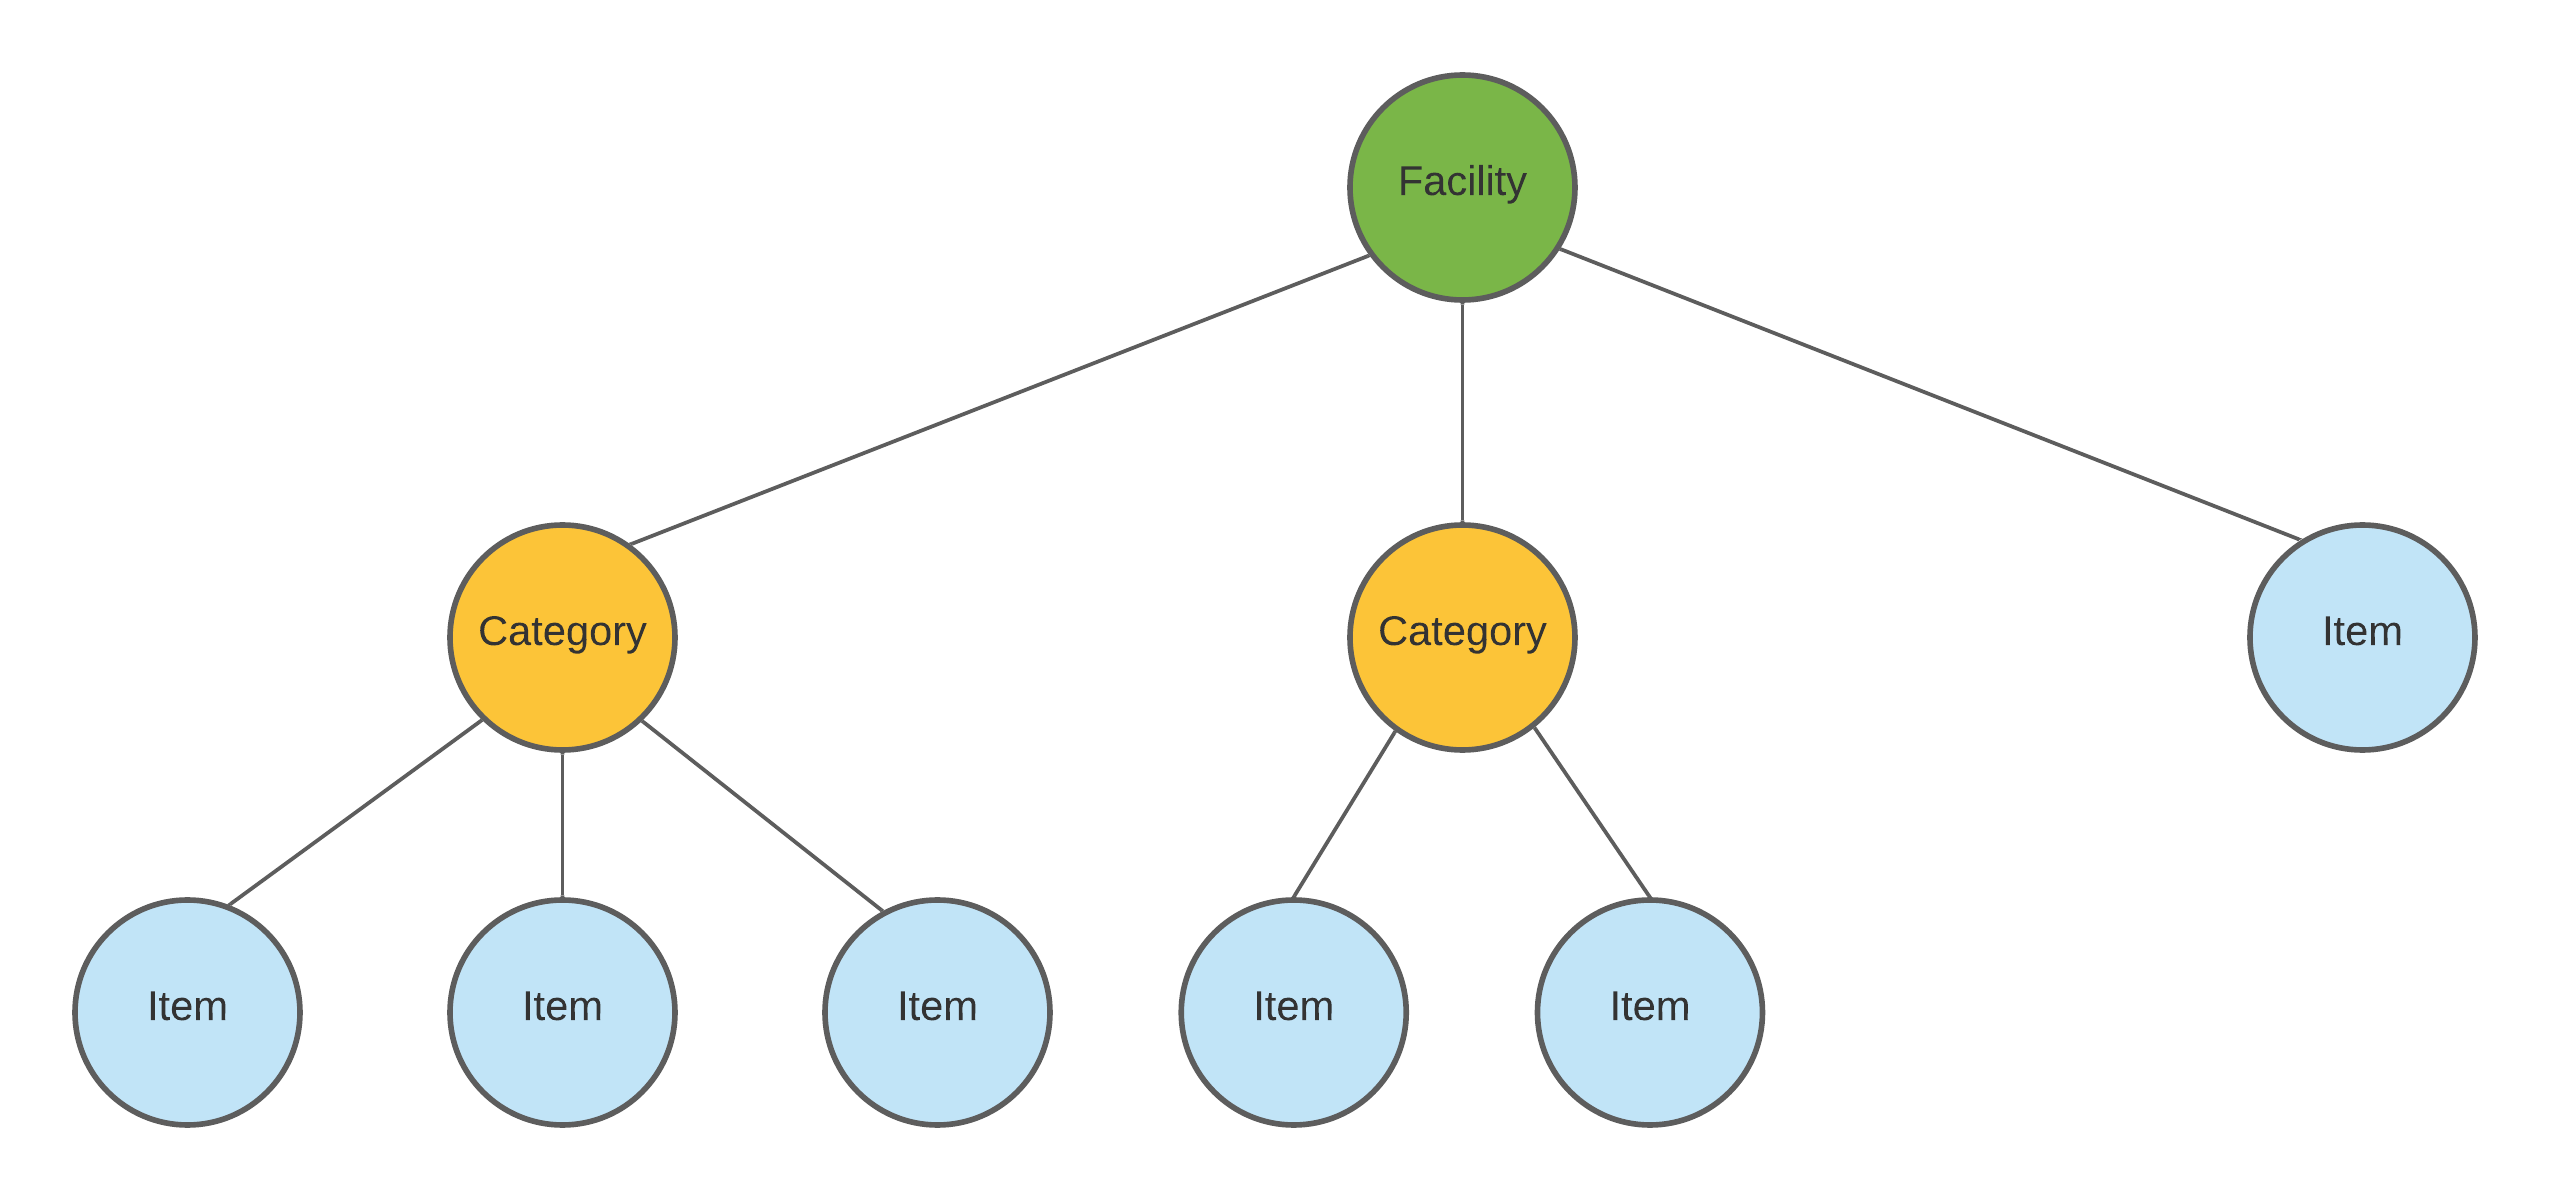
\includegraphics[scale=0.12]{images/db-overview.png}
    \caption{facility tree structure}
    \label{fig:db-overview}
\end{figure}

The user permission is based on the nodes. Any user with permission to the node has access to all the nodes under it. i.e., a user with permission on a node has access to all the nodes in the sub-tree rooted at that node. \\

The related item keeps track of the items that are closely brought or rented with one another. It is based on the Least Recently Used (LRU) cache algorithm where the least recently brought or rented together item is removed when the cache overflows.
The inventory history keeps track of the added and removed items and the item history keeps track of the brought and rented items.